% The master copy of this demo dissertation is held on my filespace
% on the cl file serve (/homes/mr/teaching/demodissert/)

% Last updated by MR on 2 August 2001

\documentclass[12pt,twoside,notitlepage]{report}

\usepackage{a4}
\usepackage{verbatim}

\input{epsf}                            % to allow postscript inclusions
% On thor and CUS read top of file:
%     /opt/TeX/lib/texmf/tex/dvips/epsf.sty
% On CL machines read:
%     /usr/lib/tex/macros/dvips/epsf.tex



\raggedbottom                           % try to avoid widows and orphans
\sloppy
\clubpenalty1000%
\widowpenalty1000%

\addtolength{\oddsidemargin}{6mm}       % adjust margins
\addtolength{\evensidemargin}{-8mm}

\renewcommand{\baselinestretch}{1.1}    % adjust line spacing to make
                                        % more readable

\begin{document}

\bibliographystyle{plain}


%%%%%%%%%%%%%%%%%%%%%%%%%%%%%%%%%%%%%%%%%%%%%%%%%%%%%%%%%%%%%%%%%%%%%%%%
% Title


\pagestyle{empty}

\hfill{\LARGE \bf Martin Richards}

\vspace*{60mm}
\begin{center}
\Huge
{\bf How to write a dissertation in \LaTeX} \\
\vspace*{5mm}
Diploma in Computer Science \\
\vspace*{5mm}
St John's College \\
\vspace*{5mm}
\today  % today's date
\end{center}

\cleardoublepage

%%%%%%%%%%%%%%%%%%%%%%%%%%%%%%%%%%%%%%%%%%%%%%%%%%%%%%%%%%%%%%%%%%%%%%%%%%%%%%
% Proforma, table of contents and list of figures

\setcounter{page}{1}
\pagenumbering{roman}
\pagestyle{plain}

\chapter*{Proforma}

{\large
\begin{tabular}{ll}
Name:               & \bf Martin Richards                       \\
College:            & \bf St John's College                     \\
Project Title:      & \bf How to write a dissertation in \LaTeX \\
Examination:        & \bf Diploma in Computer Science, July 2001        \\
Word Count:         & \bf 1587\footnotemark[1]
(well less than the 12000 limit) \\
Project Originator: & Dr M.~Richards                    \\
Supervisor:         & Dr M.~Richards                    \\ 
\end{tabular}
}
\footnotetext[1]{This word count was computed
by {\tt detex diss.tex | tr -cd '0-9A-Za-z $\tt\backslash$n' | wc -w}
}
\stepcounter{footnote}


\section*{Original Aims of the Project}

To write a demonstration dissertation\footnote{A normal footnote without the
complication of being in a table.} using \LaTeX\ to save
student's time when writing their own dissertations. The dissertation
should illustrate how to use the more common \LaTeX\ constructs. It
should include pictures and diagrams to show how these can be
incorporated into the dissertation.  It should contain the entire
\LaTeX\ source of the dissertation and the Makefile.  It should
explain how to construct an MSDOS disk of the dissertation in
Postscript format that can be used by the book shop for printing, and,
finally, it should have the prescribed layout and format of a diploma
dissertation.


\section*{Work Completed}

All that has been completed appears in this dissertation.

\section*{Special Difficulties}

Learning how to incorporate encapulated postscript into a \LaTeX\
document on both CUS and Thor.
 
\newpage
\section*{Declaration}

I, [Name] of [College], being a candidate for Part II of the Computer
Science Tripos [or the Diploma in Computer Science], hereby declare
that this dissertation and the work described in it are my own work,
unaided except as may be specified below, and that the dissertation
does not contain material that has already been used to any substantial
extent for a comparable purpose.

\bigskip
\leftline{Signed [signature]}

\medskip
\leftline{Date [date]}

\cleardoublepage

\tableofcontents

\listoffigures

\newpage
\section*{Acknowledgements}

This document owes much to an earlier version written by Simon Moore
\cite{moore95}.  His help, encouragement and advice was greatly 
appreciated.

%%%%%%%%%%%%%%%%%%%%%%%%%%%%%%%%%%%%%%%%%%%%%%%%%%%%%%%%%%%%%%%%%%%%%%%
% now for the chapters

\cleardoublepage        % just to make sure before the page numbering
                        % is changed

\setcounter{page}{1}
\pagenumbering{arabic}
\pagestyle{headings}

\chapter{Introduction}

\section{Overview of the files}

This document consists of the following files:

\begin{itemize}
\item {\tt Makefile} --- The Makefile for the dissertation and Project Proposal
\item {\tt diss.tex} --- The dissertation
\item {\tt propbody.tex} --- Appendix~C  -- the project proposal 
\item {\tt proposal.tex}  --- A \LaTeX\ main file for the proposal 
\item{\tt figs} -- A directory containing diagrams and pictures
\item{\tt refs.bib} --- The bibliography database
\end{itemize}

\section{Building the document}

This document was produced using \LaTeXe which is based upon
\LaTeX\cite{Lamport86}.  To build the document you first need to
generate {\tt diss.aux} which, amongst other things, contains the
references used.  This if done by executing the command:

{\tt latex diss}

\noindent
Then the bibliography can be generated from {\tt refs.bib} using:

{\tt bibtex diss}

\noindent
Finally, to ensure all the page numbering is correct run {\tt latex}
on {\tt diss.tex} until the {\tt .aux} files do not change.  This
usually takes 2 more runs.

\subsection{The makefile}

To simplify the calls to {\tt latex} and {\tt bibtex}, 
a makefile has been provided, see Appendix~\ref{makefile}. 
It provides the following facilities:

\begin{itemize}

\item{\tt make} \\
 Display help information.

\item{\tt make prop} \\
 Run {\tt latex proposal; xdvi proposal.dvi}.

\item{\tt make diss.ps} \\
 Make the file {\tt diss.ps}.

\item{\tt make gv} \\
 View the dissertation using ghostview after performing 
{\tt make diss.ps}, if necessary.

\item{\tt make gs} \\
 View the dissertation using ghostscript after performing 
{\tt make diss.ps}, if necessary.

\item{\tt make count} \\
Display an estimate of the word count.

\item{\tt make all} \\
Construct {\tt proposal.dvi} and {\tt diss.ps}.

\item{\tt make pub} \\ Make a {\tt .tar} version of the {\tt demodiss}
directory and place it in my {\tt public\_html} directory.

\item{\tt make clean} \\ Delete all files except the source files of
the dissertation. All these deleted files can be reconstructed by
typing {\tt make all}.

\item{\tt make pr} \\
Print the dissertation on your default printer.

\end{itemize}


\section{Counting words}

An approximate word count of the body of the dissertation may be
obtained using:

{\tt wc diss.tex}

\noindent
Alternatively, try something like:

\verb/detex diss.tex | tr -cd '0-9A-Z a-z\n' | wc -w/




\cleardoublepage



\chapter{Preparation}

This chapter is empty!


\cleardoublepage
\chapter{Implementation}

\section{Verbatim text}

Verbatim text can be included using \verb|\begin{verbatim}| and
\verb|\end{verbatim}|. I normally use a slightly smaller font and
often squeeze the lines a little closer together, as in:

{\renewcommand{\baselinestretch}{0.8}\small\begin{verbatim}
GET "libhdr"
 
GLOBAL { count:200; all  }
 
LET try(ld, row, rd) BE TEST row=all
                        THEN count := count + 1
                        ELSE { LET poss = all & ~(ld | row | rd)
                               UNTIL poss=0 DO
                               { LET p = poss & -poss
                                 poss := poss - p
                                 try(ld+p << 1, row+p, rd+p >> 1)
                               }
                             }
LET start() = VALOF
{ all := 1
  FOR i = 1 TO 12 DO
  { count := 0
    try(0, 0, 0)
    writef("Number of solutions to %i2-queens is %i5*n", i, count)
    all := 2*all + 1
  }
  RESULTIS 0
}
\end{verbatim}
}

\section{Tables}

\begin{samepage}
Here is a simple example\footnote{A footnote} of a table.

\begin{center}
\begin{tabular}{l|c|r}
Left      & Centred & Right \\
Justified &         & Justified \\[3mm]
%\hline\\%[-2mm]
First     & A       & XXX \\
Second    & AA      & XX  \\
Last      & AAA     & X   \\
\end{tabular}
\end{center}

\noindent
There is another example table in the proforma.
\end{samepage}

\section{Simple diagrams}

Simple diagrams can be written directly in \LaTeX.  For example, see
figure~\ref{latexpic1} on page~\pageref{latexpic1} and see
figure~\ref{latexpic2} on page~\pageref{latexpic2}.

\begin{figure}
\setlength{\unitlength}{1mm}
\begin{center}
\begin{picture}(125,100)
\put(0,80){\framebox(50,10){AAA}}
\put(0,60){\framebox(50,10){BBB}}
\put(0,40){\framebox(50,10){CCC}}
\put(0,20){\framebox(50,10){DDD}}
\put(0,00){\framebox(50,10){EEE}}

\put(75,80){\framebox(50,10){XXX}}
\put(75,60){\framebox(50,10){YYY}}
\put(75,40){\framebox(50,10){ZZZ}}

\put(25,80){\vector(0,-1){10}}
\put(25,60){\vector(0,-1){10}}
\put(25,50){\vector(0,1){10}}
\put(25,40){\vector(0,-1){10}}
\put(25,20){\vector(0,-1){10}}

\put(100,80){\vector(0,-1){10}}
\put(100,70){\vector(0,1){10}}
\put(100,60){\vector(0,-1){10}}
\put(100,50){\vector(0,1){10}}

\put(50,65){\vector(1,0){25}}
\put(75,65){\vector(-1,0){25}}
\end{picture}
\end{center}
\caption{\label{latexpic1}A picture composed of boxes and vectors.}
\end{figure}

\begin{figure}
\setlength{\unitlength}{1mm}
\begin{center}

\begin{picture}(100,70)
\put(47,65){\circle{10}}
\put(45,64){abc}

\put(37,45){\circle{10}}
\put(37,51){\line(1,1){7}}
\put(35,44){def}

\put(57,25){\circle{10}}
\put(57,31){\line(-1,3){9}}
\put(57,31){\line(-3,2){15}}
\put(55,24){ghi}

\put(32,0){\framebox(10,10){A}}
\put(52,0){\framebox(10,10){B}}
\put(37,12){\line(0,1){26}}
\put(37,12){\line(2,1){15}}
\put(57,12){\line(0,2){6}}
\end{picture}

\end{center}
\caption{\label{latexpic2}A diagram composed of circles, lines and boxes.}
\end{figure}



\section{Adding more complicated graphics}

The use of \LaTeX\ format can be tedious and it is often better to use
encapsulated postscript to represent complicated graphics.
Figure~\ref{epsfig} and ~\ref{xfig} on page \pageref{xfig} are
examples. The second figure was drawn using {\tt xfig} and exported in
{\tt.eps} format. This is my recommended way of drawing all diagrams.


\begin{figure}[tbh]
\centerline{\epsfbox{figs/cuarms.eps}}
\caption{\label{epsfig}Example figure using encapsulated postscript}
\end{figure}

\begin{figure}[tbh]
\vspace{4in}
\caption{\label{pastedfig}Example figure where a picture can be pasted in}
\end{figure}


\begin{figure}[tbh]
\centerline{\epsfbox{figs/diagram.eps}}
\caption{\label{xfig}Example diagram drawn using {\tt xfig}}
\end{figure}




\cleardoublepage
\chapter{Evaluation}

\section{Printing and binding}

If you have access to a laser printer that can print on two sides, you
can use it to print two copies of your dissertation and then get them
bound by the Computer Laboratory Bookshop. Otherwise, print your
dissertation single sided and get the Bookshop to copy and bind it double
sided.


Better printing quality can sometimes be obtained by giving the
Bookshop an MSDOS 1.44~Mbyte 3.5" floppy disc containing the
Postscript form of your dissertation. If the file is too large a
compressed version with {\tt zip} but not {\tt gnuzip} nor {\tt
compress} is acceptable. However they prefer the uncompressed form if
possible. From my experience I do not recommend this method.

\subsection{Things to note}

\begin{itemize}
\item Ensure that there are the correct number of blank pages inserted
so that each double sided page has a front and a back.  So, for
example, the title page must be followed by an absolutely blank page
(not even a page number).

\item Submitted postscript introduces more potential problems.
Therefore you must either allow two iterations of the binding process
(once in a digital form, falling back to a second, paper, submission if
necessary) or submit both paper and electronic versions.

\item There may be unexpected problems with fonts.

\end{itemize}

\section{Further information}

See the Computer Lab's world wide web pages at URL:

{\tt http://www.cl.cam.ac.uk/TeXdoc/TeXdocs.html}


\cleardoublepage
\chapter{Conclusion}

I hope that this rough guide to writing a dissertation is \LaTeX\ has
been helpful and saved you time.




\cleardoublepage

%%%%%%%%%%%%%%%%%%%%%%%%%%%%%%%%%%%%%%%%%%%%%%%%%%%%%%%%%%%%%%%%%%%%%
% the bibliography

\addcontentsline{toc}{chapter}{Bibliography}
\bibliography{refs}
\cleardoublepage

%%%%%%%%%%%%%%%%%%%%%%%%%%%%%%%%%%%%%%%%%%%%%%%%%%%%%%%%%%%%%%%%%%%%%
% the appendices
\appendix

\chapter{Latex source}

\section{diss.tex}
{\scriptsize\verbatiminput{diss.tex}}

\section{proposal.tex}
{\scriptsize\verbatiminput{proposal.tex}}

\section{propbody.tex}
{\scriptsize\verbatiminput{propbody.tex}}



\cleardoublepage

\chapter{Makefile}

\section{\label{makefile}Makefile}
{\scriptsize\verbatiminput{makefile.txt}}

\section{refs.bib}
{\scriptsize\verbatiminput{refs.bib}}


\cleardoublepage

\chapter{Project Proposal}



\title{Machine learning inference of search engine heuristics}
\subtitle{Part II Computer Science Project Proposal}
\author{K. Palyutina, St. Catharine's College \\
        Originator: Dr. Jon Crowcroft}


% Main document

\section*{\bf Introduction, The Problem To Be Addressed}
PageRank (an algorithm which is used by Google to evaluate the `importance' of a web page) is one of the most crucial factors which determine page performance in search returns. However, there are many more of such factors that are believed to become increasingly influential. Because Google's algorithm is frequently revised, changing page ranks cause web site owners to speculate about how their web pages `deserved' an upgrade or a downgrade. Despite a large interest in this area, little research has been done to determine to what degree such factors affect the performance of a page. Certain tools\footnote{For example, Woorank or SEO are the most popular Chrome extensions to assess certain page qualities.} exist which attempt to advise web masters how to `improve' their pages. However, heuristics used by such tools are not known and are possibly incomplete and no attempt has come close to accurately predicting Google rankings.

A problem of approximating algorithms which may be used by modern search engines is characterised by vast search space, which makes exhaustive search impossible and introduces the need for generalisation. Such a problem can be reduced to a classification problem, which is traditionally solved with the help of machine learning techniques. Even though machine learning finds natural application in this area, it is easy to see how it would be very hard to create a learner and apply it to, for example, Google's search engine. Naturally, one would need to have exhaustive resources to conduct such a study. Besides, machine learning has major drawbacks that would hinder such an ambitious experiment.

Firstly, there are little theoretical guarantees in this approach. Bounds, if any, referring to how much data needs to be processed to produce a `correct' classifier are very imprecise and a classifier that performs well in practice may not be `true'\footnote{A classifier is `true' if it classifies data correctly for all inputs.}. This means that if a machine learner was to be trained by the `real world' data (Google search returns), little could be said about the performance of the obtained algorithm or, indeed, the `truthfulness' of it. Not only would it give little insight into how successful the learning is, but also no guidance for improvement. 

Another similar issue is referred to as `overfitting': this describes a situation in which a classifier performs outstandingly on a particular set of data (often similar to training data), but given different data will perform as badly as random selection. This occurs when false connections between features and outputs have been made by the learner. Unfortunately, there is no single technique that will always avoid over/under-fitting\cite{domingos}.

Clearly, such limitations are hard to combat. Besides, machine learning techniques vary greatly, so clear and detailed feedback is essential to draw conclusions about the performance of a learner. Knowing how a particular technique copes with certain heuristics would be valuable, as it would allow to approach the original problem (approximating search engine heuristics reliably) in an informed way.  

In this light, this project aspires to explore how machine learning techniques can be used to infer algorithms from search engines. To battle the constraints described above I will write my own simple search engine which will be used to observe the effectiveness of different machine learning techniques (see Figure \ref{diag1}). The existence of such a search engine is vital to the project, as it offers ultimate control over the learning process. The heuristics used in the search engine will be transparent, which, for example, eliminates the dependency on continuously changing heuristics used by Google. Another advantage of this approach is the fact that only a minimal fraction of the web needs to be used. Such a `mini-internet' will reside offline, which will speed up the indexing and also allow local modification of web pages. 

\begin{figure}
\centering
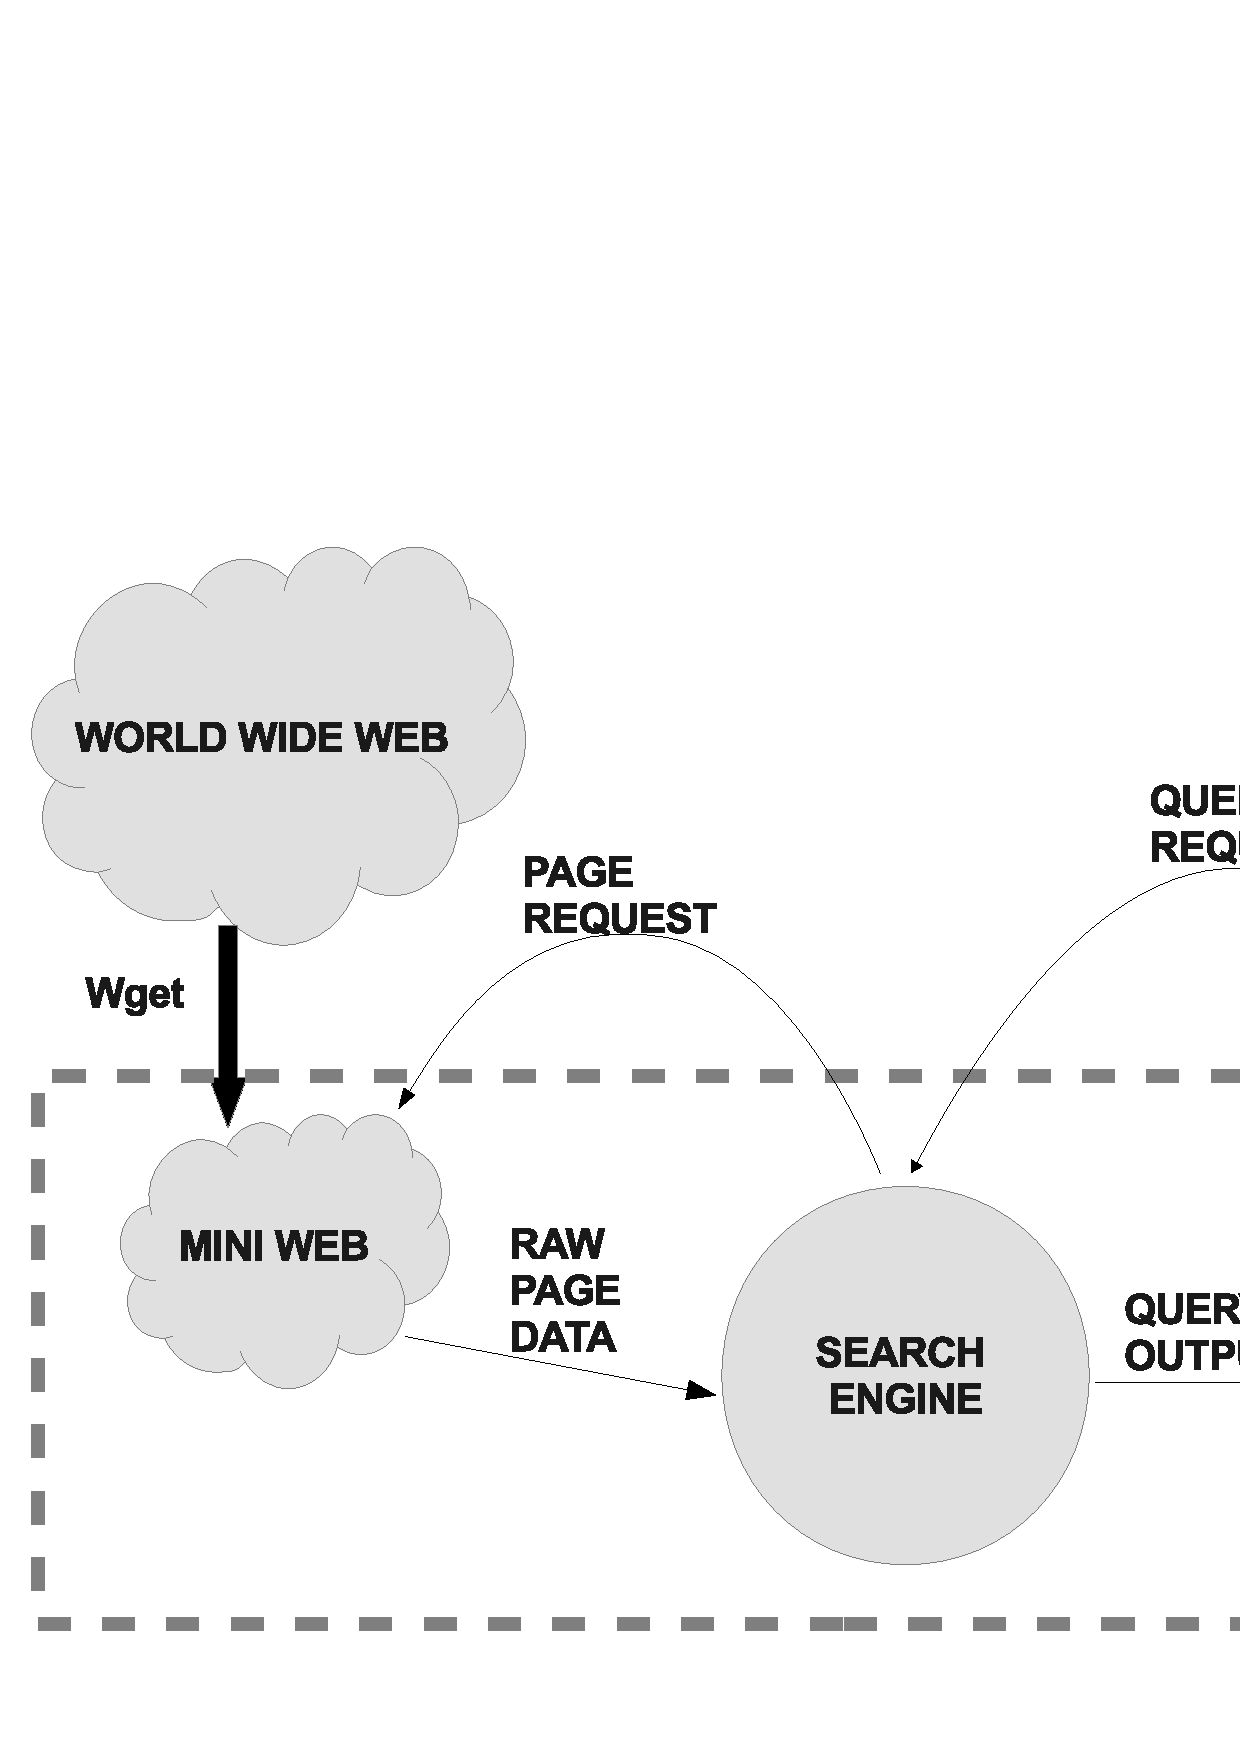
\includegraphics[scale=0.5]{diagram1}
\caption{The training of the learner. The system enclosed within the dotted box will be implemented in this project. The mini web is created by cloning web pages from the internet. The learner queries the search engine and gets back the results of the query as an input. }
\label{diag1}
\end{figure}

Most importantly, this approach gives me straightforward ways to reason about the performance of learning techniques. The search engine can be evolved to incorporate various heuristics together with PageRank. Such heuristics need not match Google's actual heuristics, however must aim to improve browsing experience \footnote{`Precision and Recall' method can be used as a guide to evaluation of search engine complexity.}. A lot of speculation has been done by web masters as to which qualities of a web page affect its ranking, these include compliance with web standards, number of words per page, frequency of occurrence of the search term on the page and alike. Because the goal of the project does not include `reverse engineering' any particular existing algorithm, there is no harm in using such guesses as guidance. 

Evolving the search engine and, hence, the learner iteratively will result in comprehensive conclusions about the effectiveness of the machine learning technique in question. Such conclusions can be used in the future as a guidance to learner design. 

\section*{\bf Starting Point}

\begin{itemize}
\item A project\footnote{\url{http://www.scienceforsearch.com/project1.asp}} was undertaken by the proposer, which developed a primitive algorithm to predict, given six characteristics of a web page, its Google ranking.  This project is mainly an inspiration, however, the speculations about the Google page ranking factors can be useful for the search engine design. 
\item Python packages exist for manipulating web pages.
\item Wget is a Linux open source utility that can be used to clone web pages.
\item The paper describing PageRank is published and will be used to implement the algorithm.
\end{itemize}


\section*{\bf Resources Required}
\begin{itemize}
\item For this project I shall mainly use my own dual-core computer that runs Ubuntu Linux. I accept full responsibility for this machine and I have made contingency plans to protect myself against hardware and/or software failure.
\item Backup will be to a BitBucket repository and/or an external hard drive.
\item I will work on MCS computers should my main machine suddenly fail. 
\end{itemize}
\section*{\bf Work to be done}

The project breaks down into the following sub-projects:

\begin{enumerate}
\item Decide on a category of search terms to explore in order to create a small network consisting of relevant web pages.

\item Implement PageRank within this network. 

\item Write a simple search engine incorporating PageRank and few other features. 

\item Decide on the representation of the input for the learner and set up the framework to format it. 

\item In advance set aside training and test data: this is necessary to then justify the evaluation of the classifier.

\item Write a simple prototype for the learner\footnote {A Naive Bayesian would be a good prototype to use.} to test the grounds. Evaluate its performance to then set goals for the final learner.  

\item Design, implement and test the learner. 

\item Attempt to evolve the search engine to be more usable and complex and observe how the learner copes with the changes of the search engine. 


\end{enumerate}

\section*{\bf Success Criterion for the Main Result}


The project will be a success if... 
\begin{itemize}
\item The resulting classifier can identify the importance of the PageRank factor in the given search engine.
\item The results of the experiment show how the chosen machine learning technique deals with various search engine heuristics. I would especially like to observe that certain heuristics are harder to pick up on than others and vice versa.
\end{itemize}
\section*{\bf Possible Extensions}
If I achieve my main result early I shall experiment with other machine learning techniques to see which perform better. I could also apply my learner to real search engines such as Google and Bing in the hope of 
discovering dependencies between features of the page and its success in ranking results.
\section*{\bf Timetable: Work plan and Milestones to be achieved.}


Planned starting date is 19/10/2011.

\begin{enumerate}

\item {\bf 9 Oct - 19 Oct:} 
\begin{itemize}
\item Do preliminary reading.
\item Familiarize myself with the field of machine learning.
\end{itemize} 
{\bf Milestone: } Complete project proposal. 
\item {\bf Oct 20 - Nov 3:} 
    \begin{itemize}
    \item Decide which and how many websites should be cloned for use as the mini web.  
    \item Prepare some training data and, separately, test data. This includes queries to be run on the search engine and expected results. 
    \end{itemize}
\item {\bf Nov 4 - Nov 15:} 
    \begin{itemize}
    \item Start writing a simple search engine and evaluate it on the test data. 
    \end{itemize}
\item {\bf Nov 15 - Nov 25:} 
    \begin{itemize}
    \item Finish the search engine.
    \item Start developing an early prototype for the learner. 
    \end{itemize} 
    {\bf Milestone: } Have a prototype of a complete system.
\item {\bf Nov 25 - Dec 15:} 
\begin{itemize}
\item Evaluate the performance of the prototype learner. 
\item Design and start implementing the final learner using the results obtained from the prototype as guidance. 
\end{itemize}
\item {\bf Dec 16 - Jan 1:} Finish the implementation of the learner. 
\item {\bf Jan 2 - Jan 16:} 
     Evaluate the resulting classifier. Here is also good time to try a different design for the learner if the classifier does not perform as well as intended.
\item {\bf Jan 17 - Feb 1:} Start working on progress report.  
{Milestone: } Write progress report. 
\item {\bf Feb 2 - Feb 20} Implement extensions.

\item {\bf Feb 20 - Mar 5:} Evaluate extensions. 

\item {\bf Mar 5 - Mar 25:} Write dissertation main chapters.

\item {\bf Mar 25 - April 10}  Further evaluation and complete dissertation.
{Milestone: } Dissertation final draft is finished.

\item {\bf April 11 - April 20:} Proof reading and submission.

\end{enumerate}


 



\end{document}
